% Options for packages loaded elsewhere
\PassOptionsToPackage{unicode}{hyperref}
\PassOptionsToPackage{hyphens}{url}
%
\documentclass[
  ignorenonframetext,
]{beamer}
\usepackage{pgfpages}
\setbeamertemplate{caption}[numbered]
\setbeamertemplate{caption label separator}{: }
\setbeamercolor{caption name}{fg=normal text.fg}
\beamertemplatenavigationsymbolsempty
% Prevent slide breaks in the middle of a paragraph
\widowpenalties 1 10000
\raggedbottom
\setbeamertemplate{part page}{
  \centering
  \begin{beamercolorbox}[sep=16pt,center]{part title}
    \usebeamerfont{part title}\insertpart\par
  \end{beamercolorbox}
}
\setbeamertemplate{section page}{
  \centering
  \begin{beamercolorbox}[sep=12pt,center]{part title}
    \usebeamerfont{section title}\insertsection\par
  \end{beamercolorbox}
}
\setbeamertemplate{subsection page}{
  \centering
  \begin{beamercolorbox}[sep=8pt,center]{part title}
    \usebeamerfont{subsection title}\insertsubsection\par
  \end{beamercolorbox}
}
\AtBeginPart{
  \frame{\partpage}
}
\AtBeginSection{
  \ifbibliography
  \else
    \frame{\sectionpage}
  \fi
}
\AtBeginSubsection{
  \frame{\subsectionpage}
}
\usepackage{amsmath,amssymb}
\usepackage{iftex}
\ifPDFTeX
  \usepackage[T1]{fontenc}
  \usepackage[utf8]{inputenc}
  \usepackage{textcomp} % provide euro and other symbols
\else % if luatex or xetex
  \usepackage{unicode-math} % this also loads fontspec
  \defaultfontfeatures{Scale=MatchLowercase}
  \defaultfontfeatures[\rmfamily]{Ligatures=TeX,Scale=1}
\fi
\usepackage{lmodern}
\usetheme[]{Dresden}
\usecolortheme{beaver}
\usefonttheme{structurebold}
\ifPDFTeX\else
  % xetex/luatex font selection
\fi
% Use upquote if available, for straight quotes in verbatim environments
\IfFileExists{upquote.sty}{\usepackage{upquote}}{}
\IfFileExists{microtype.sty}{% use microtype if available
  \usepackage[]{microtype}
  \UseMicrotypeSet[protrusion]{basicmath} % disable protrusion for tt fonts
}{}
\makeatletter
\@ifundefined{KOMAClassName}{% if non-KOMA class
  \IfFileExists{parskip.sty}{%
    \usepackage{parskip}
  }{% else
    \setlength{\parindent}{0pt}
    \setlength{\parskip}{6pt plus 2pt minus 1pt}}
}{% if KOMA class
  \KOMAoptions{parskip=half}}
\makeatother
\usepackage{xcolor}
\newif\ifbibliography
\setlength{\emergencystretch}{3em} % prevent overfull lines
\providecommand{\tightlist}{%
  \setlength{\itemsep}{0pt}\setlength{\parskip}{0pt}}
\setcounter{secnumdepth}{-\maxdimen} % remove section numbering
\usepackage{subfig}
\AtBeginSection{}
\titlegraphic{
\includegraphics[width = 3cm]{images/unibo-logo.pdf}}
\ifLuaTeX
  \usepackage{selnolig}  % disable illegal ligatures
\fi
\IfFileExists{bookmark.sty}{\usepackage{bookmark}}{\usepackage{hyperref}}
\IfFileExists{xurl.sty}{\usepackage{xurl}}{} % add URL line breaks if available
\urlstyle{same}
\hypersetup{
  pdftitle={Predictive Modeling of NBA Game Outcomes},
  pdfauthor={Matteo Mazzarelli},
  hidelinks,
  pdfcreator={LaTeX via pandoc}}

\title{Predictive Modeling of NBA Game Outcomes}
\subtitle{Using shot efficiency as a predictor for basketball game
results}
\author{Matteo Mazzarelli}
\date{14 July 2023}

\begin{document}
\frame{\titlepage}

\hypertarget{introduction}{%
\section{Introduction}\label{introduction}}

\begin{frame}{Introduction}
The NBA has undergone a significant transformation towards data-driven
decision-making, influenced by the broader trend in various industries.
This thesis explores how the NBA's evolution has been shaped by data
analytics, with a focus on shooting strategies. It draws inspiration
from Moreyball, the playing strategy that Daryl Morey, an important
figure in NBA basketball, helped popularize. The project aims to
establish a quantitative relationship between efficient shot selection
and team success.
\end{frame}

\begin{frame}{Data under study}
\protect\hypertarget{data-under-study}{}
This thesis analyzes a comprehensive collection of basketball
statistics, including shot coordinates, game results, and player
statistics, sourced primarily from the official NBA statistics API.

\begin{itemize}
\item
  \emph{NBA Shots dataset}: A dataset spanning 2004 to 2023 which
  provides shot details from NBA games.
\item
  \emph{NBA Games dataset}: A dataset capturing team-based game results
  over the past 20 seasons.
\item
  \emph{NBA Games Details dataset}: A dataset that contains player
  statistics for each game in the games dataset.
\end{itemize}
\end{frame}

\hypertarget{exploratory-data-analysis}{%
\section{Exploratory data analysis}\label{exploratory-data-analysis}}

\begin{frame}{Exploratory data analysis}
Exploratory data analysis involves intersecting and cross-checking
multiple datasets to extract features relevant to our analysis, which
involves studying different aspects of shooting data from NBA games,
analyzing shot efficiency, and understanding the importance of shot
selection in winning games.
\end{frame}

\begin{frame}{3-point field goals}
\protect\hypertarget{point-field-goals}{}
Our initial focus was on the 3-point field goals over the past 20
seasons. The count of shot attempts and the ratio of three-point
attempts to total attempts were calculated. This data was filtered to
only include three-point shot information, and the shot results were
labeled as ``Made'' (successful shots) or ``Missed'' (unsuccessful
shots). As it shows, there has been a significant increase in the
relative frequency of 3-point attempts to total attempts over time,
meaning that increasing 3 point shooting has been identified as a
sensible strategy.
\end{frame}

\begin{frame}
\begin{figure}

{\centering 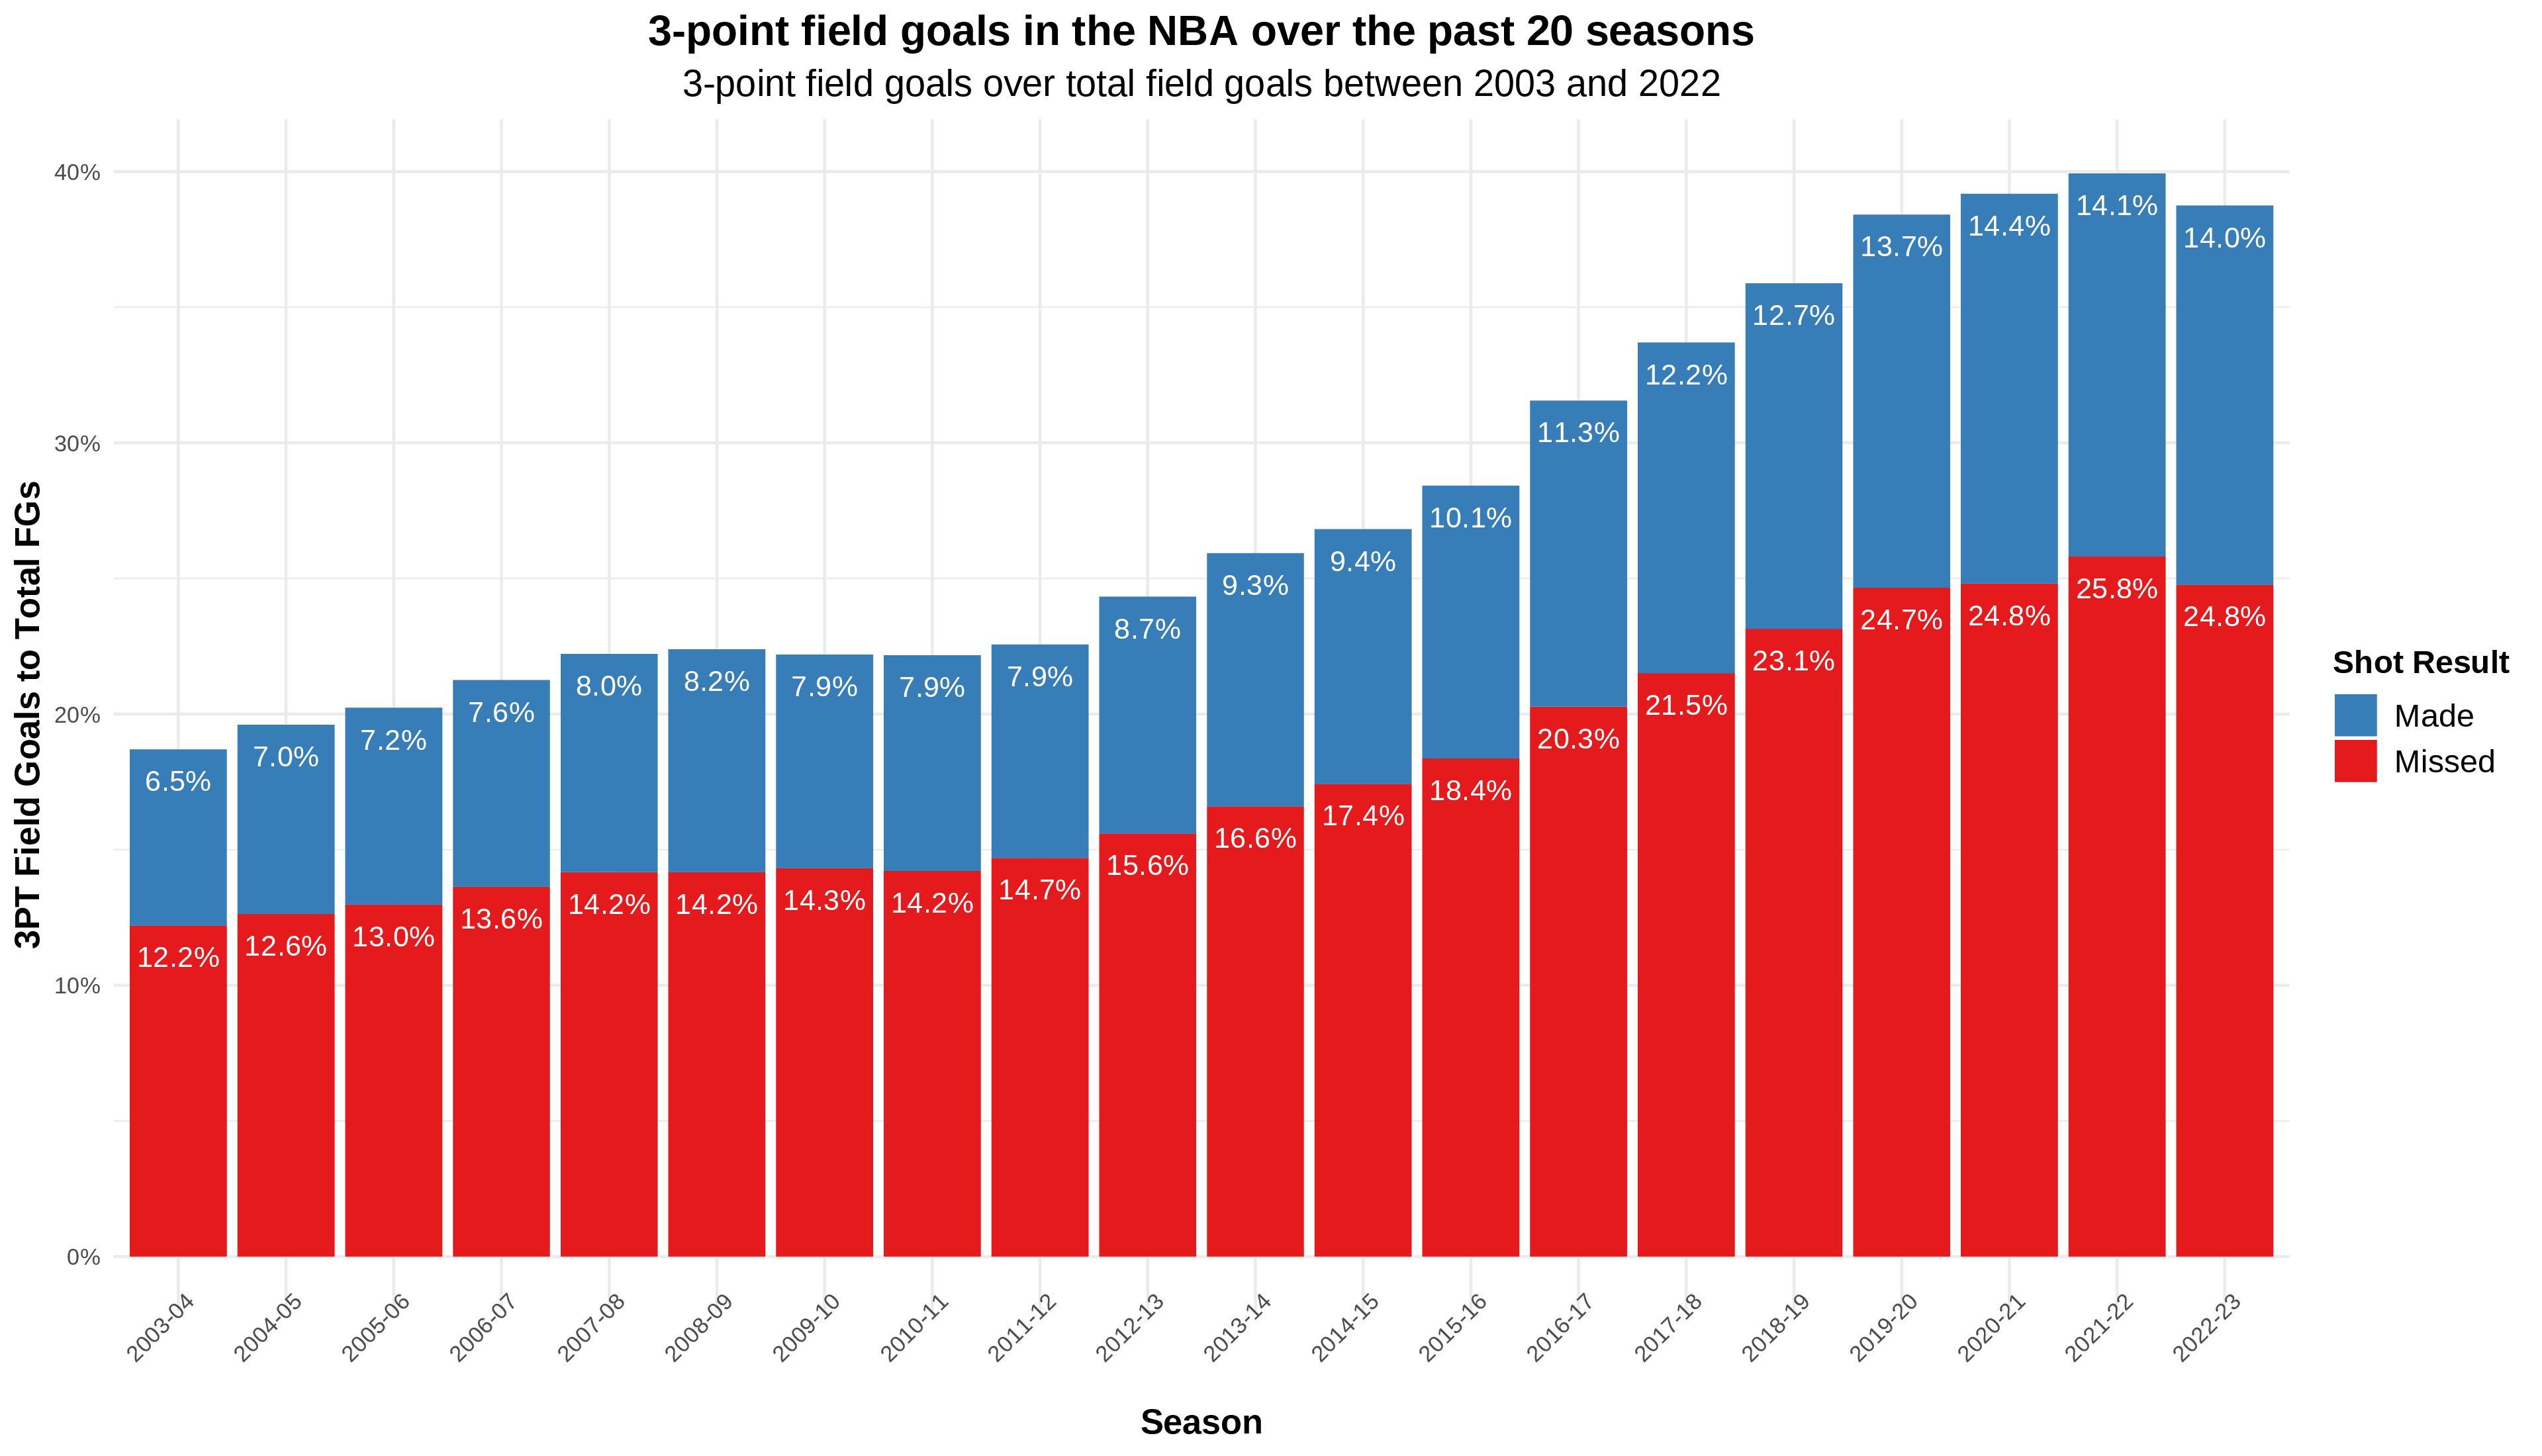
\includegraphics[width=1\linewidth]{latex/plotspres/plot_1} 

}

\caption{3-point field goals over total field goals (2003-04 to 2022-23)}\label{fig:3ptprog}
\end{figure}
\end{frame}

\begin{frame}[fragile]{The Expected Value statistic}
\protect\hypertarget{the-expected-value-statistic}{}
We computed the expected value (\texttt{EV}) of a shot in each court
area as the probability of success multiplied by its point value.

\begin{table}[H]

\caption{\label{tab:evinfo}Expected values of shots
                 taken from each area of the court}
\centering
\begin{tabular}[t]{l|r}
\hline
Court Area & EV\\
\hline
Restricted Area & 1.227\\
Right Corner 3 & 1.164\\
Left Corner 3 & 1.159\\
Above the Break 3 & 1.052\\
In The Paint (Non-RA) & 0.813\\
Mid-Range & 0.797\\
Backcourt & 0.075\\
\hline
\end{tabular}
\end{table}
\end{frame}

\begin{frame}
We computed the average expected value per shot for each season and
displayed it in a line chart, proving how teams have actively
implemented strategies that facilitate statistically efficient shooting.

\begin{figure}

{\centering 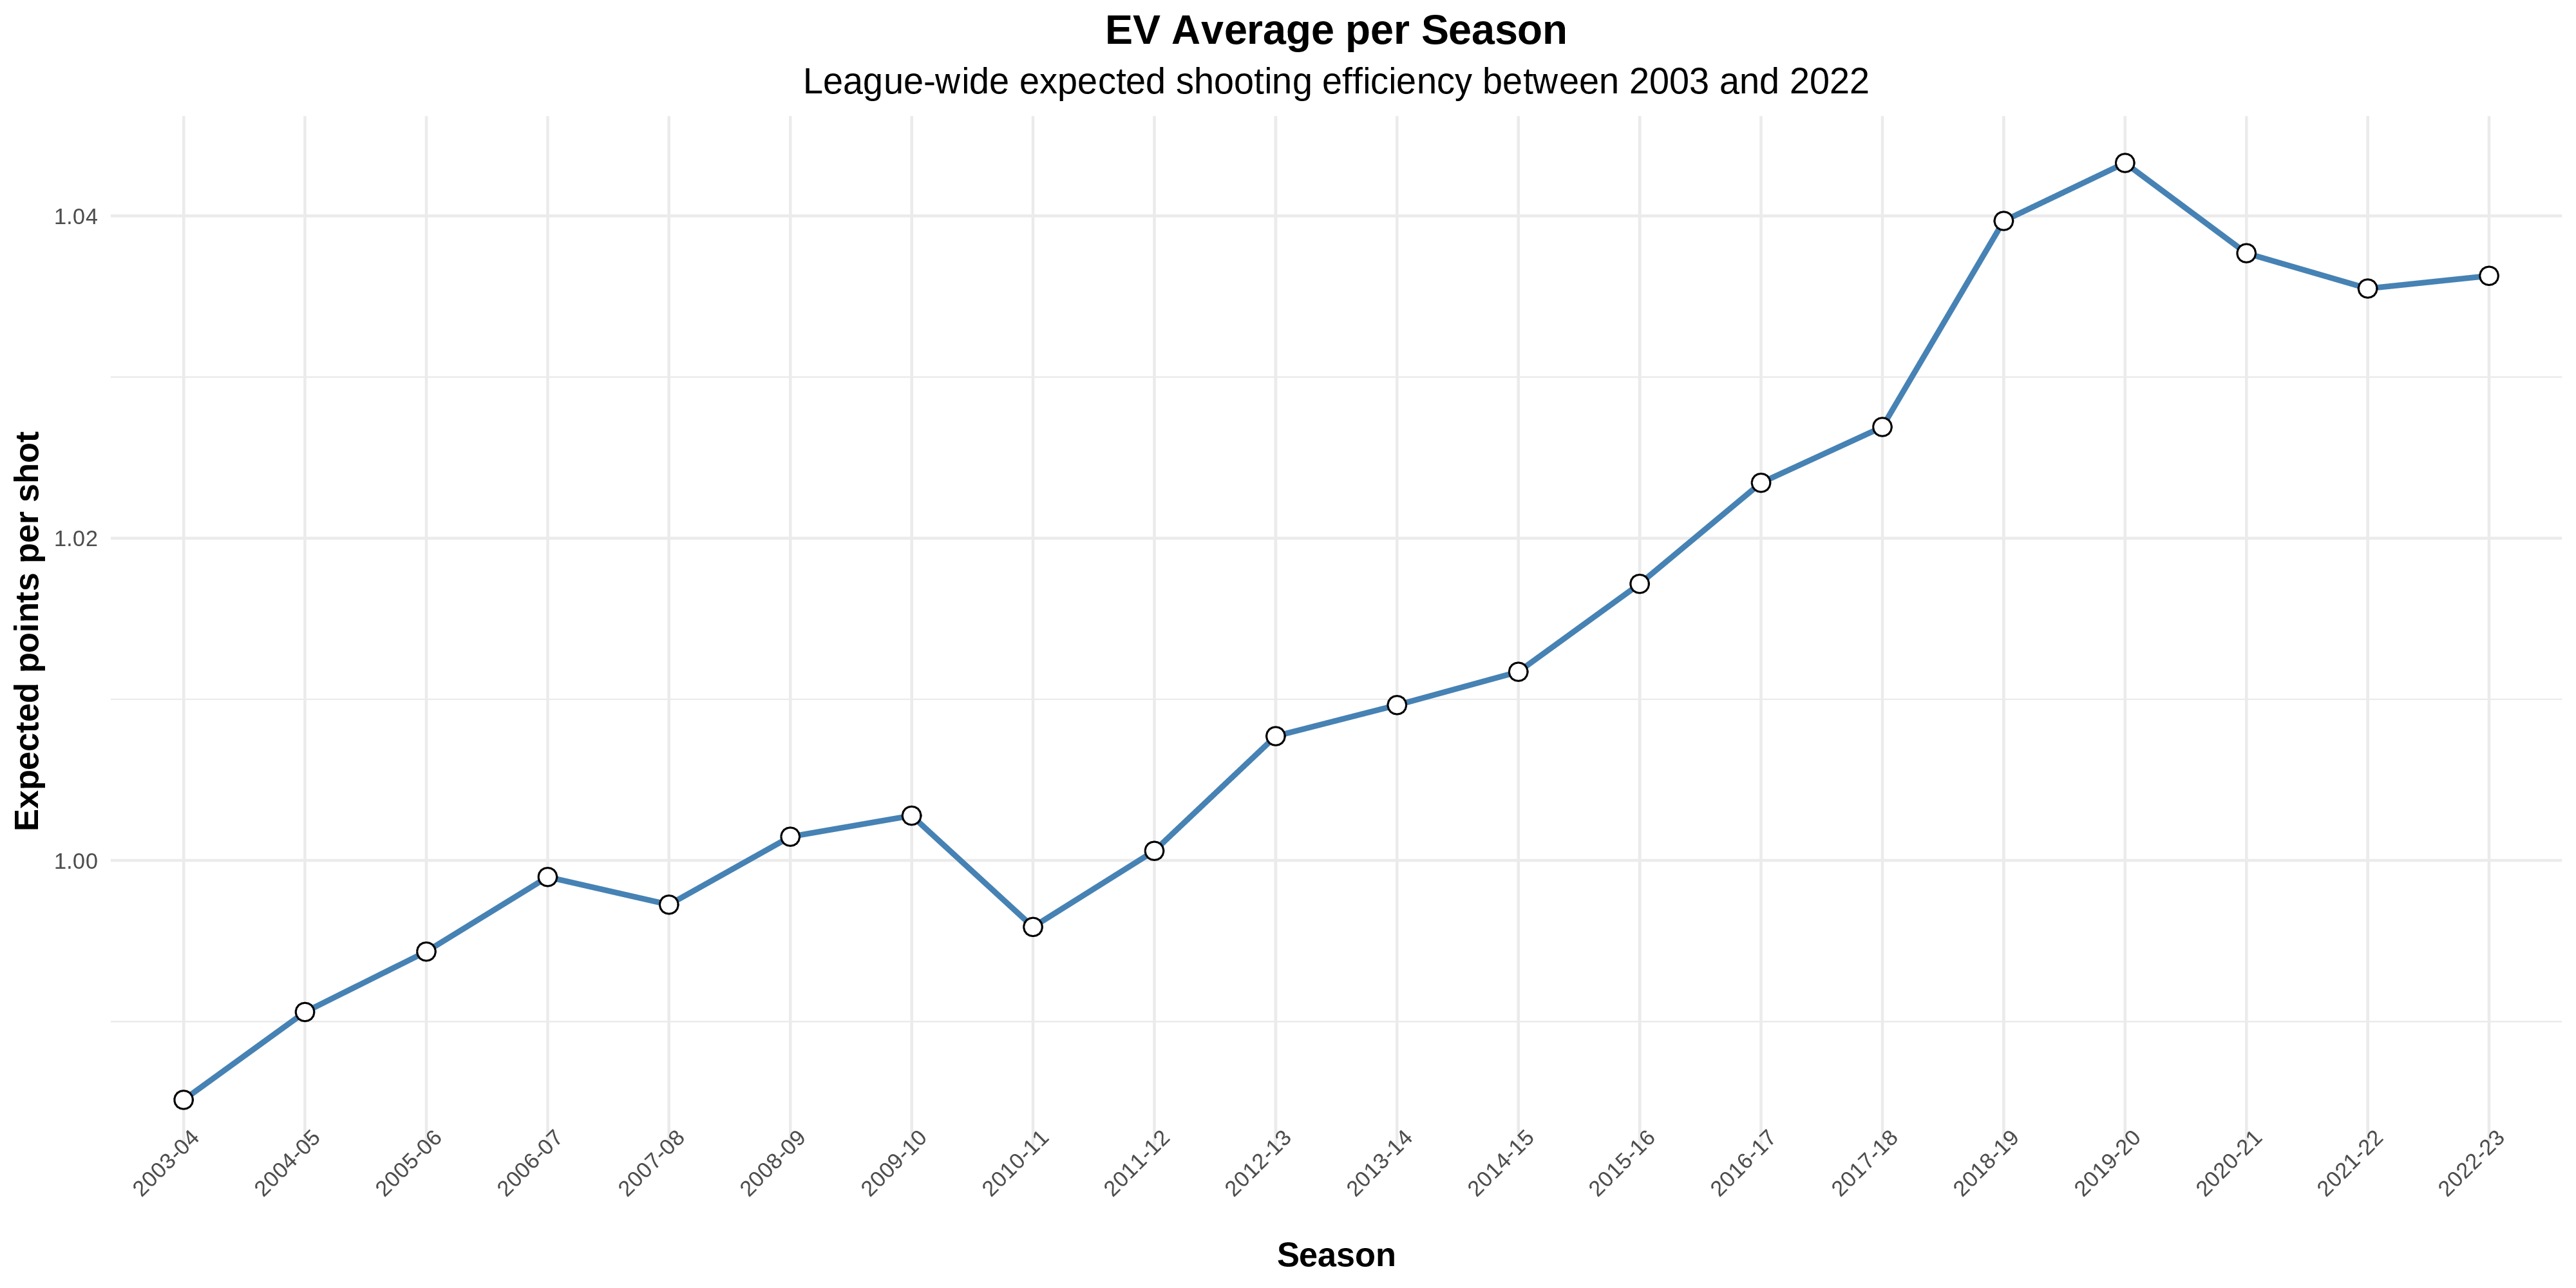
\includegraphics[width=1\linewidth]{latex/plotspres/plot_2} 

}

\caption{Expected shooting efficiency (2003-04 to 2022-23)}\label{fig:evprog}
\end{figure}
\end{frame}

\begin{frame}
Teams have been moving from a heavy reliance on mid-range shooting,
towards a bigger emphasis on 3-pointers and shots closer to the
restricted area, the most efficient shooting zone. The Houston Rockets,
shown below, have been led to great results by Daryl Morey's data-driven
approach.

\begin{figure}

{\centering 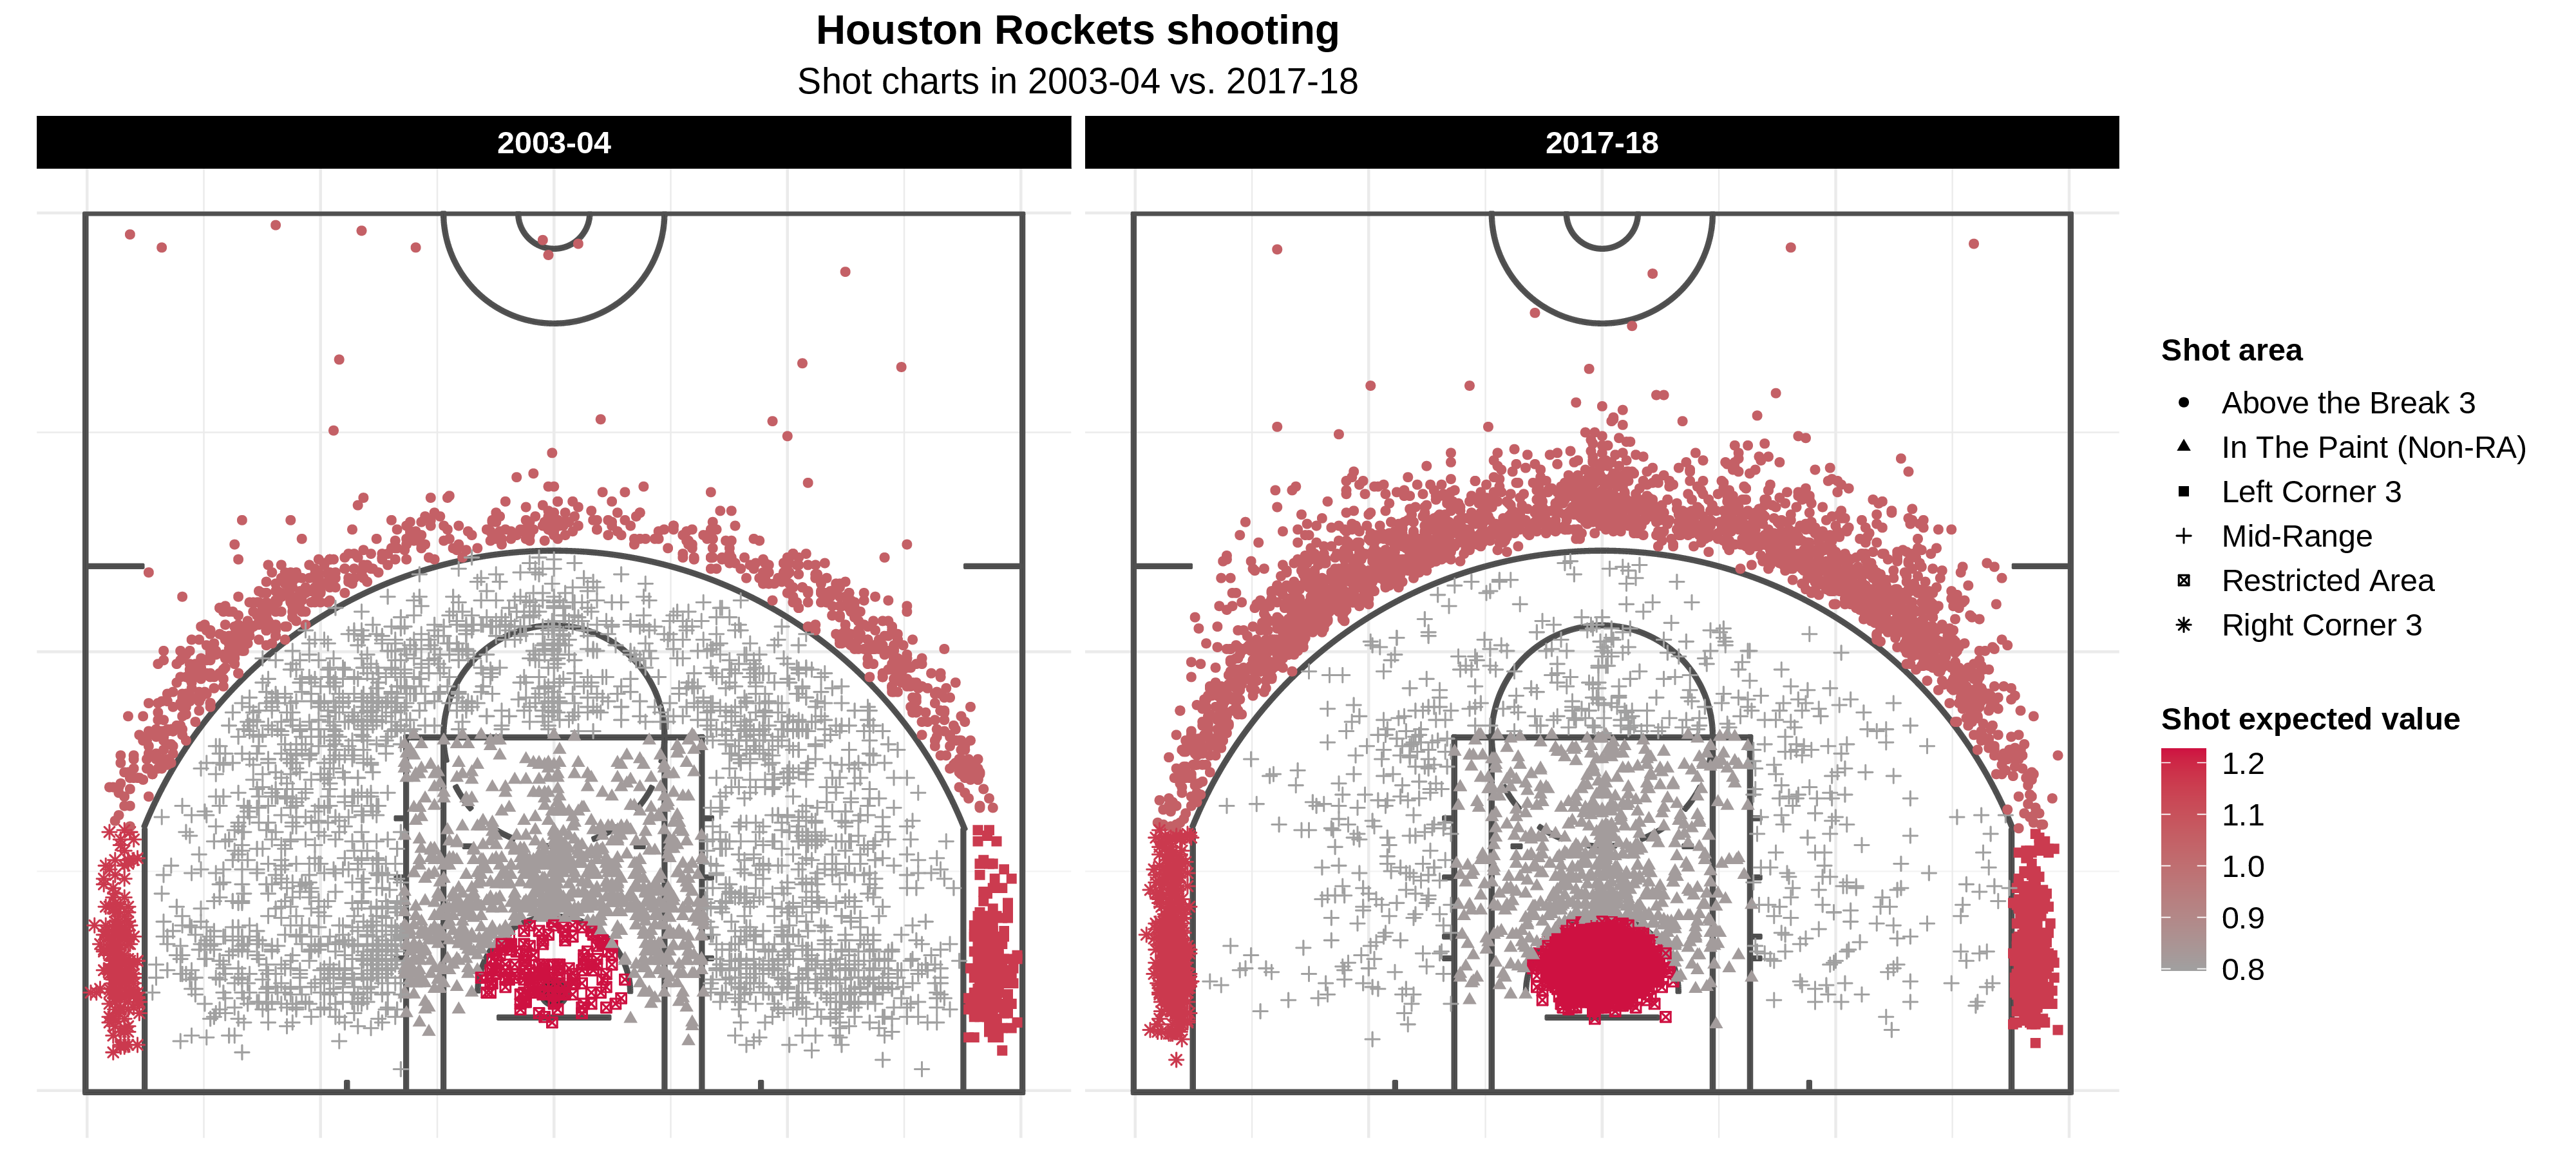
\includegraphics[width=0.9\linewidth]{latex/plotspres/plot_4} 

}

\caption{Houston Rockets shooting charts in 2003-04 and 2017-18}\label{fig:rockets}
\end{figure}
\end{frame}

\begin{frame}
As we can see from the relationship between shot precision and game
results, we can expect that including field goal accuracy statistics
will make for extremely accurate game prediction.

\begin{figure}

{\centering \subfloat[Shot precision relationship with game results\label{fig:fgpred-1}]{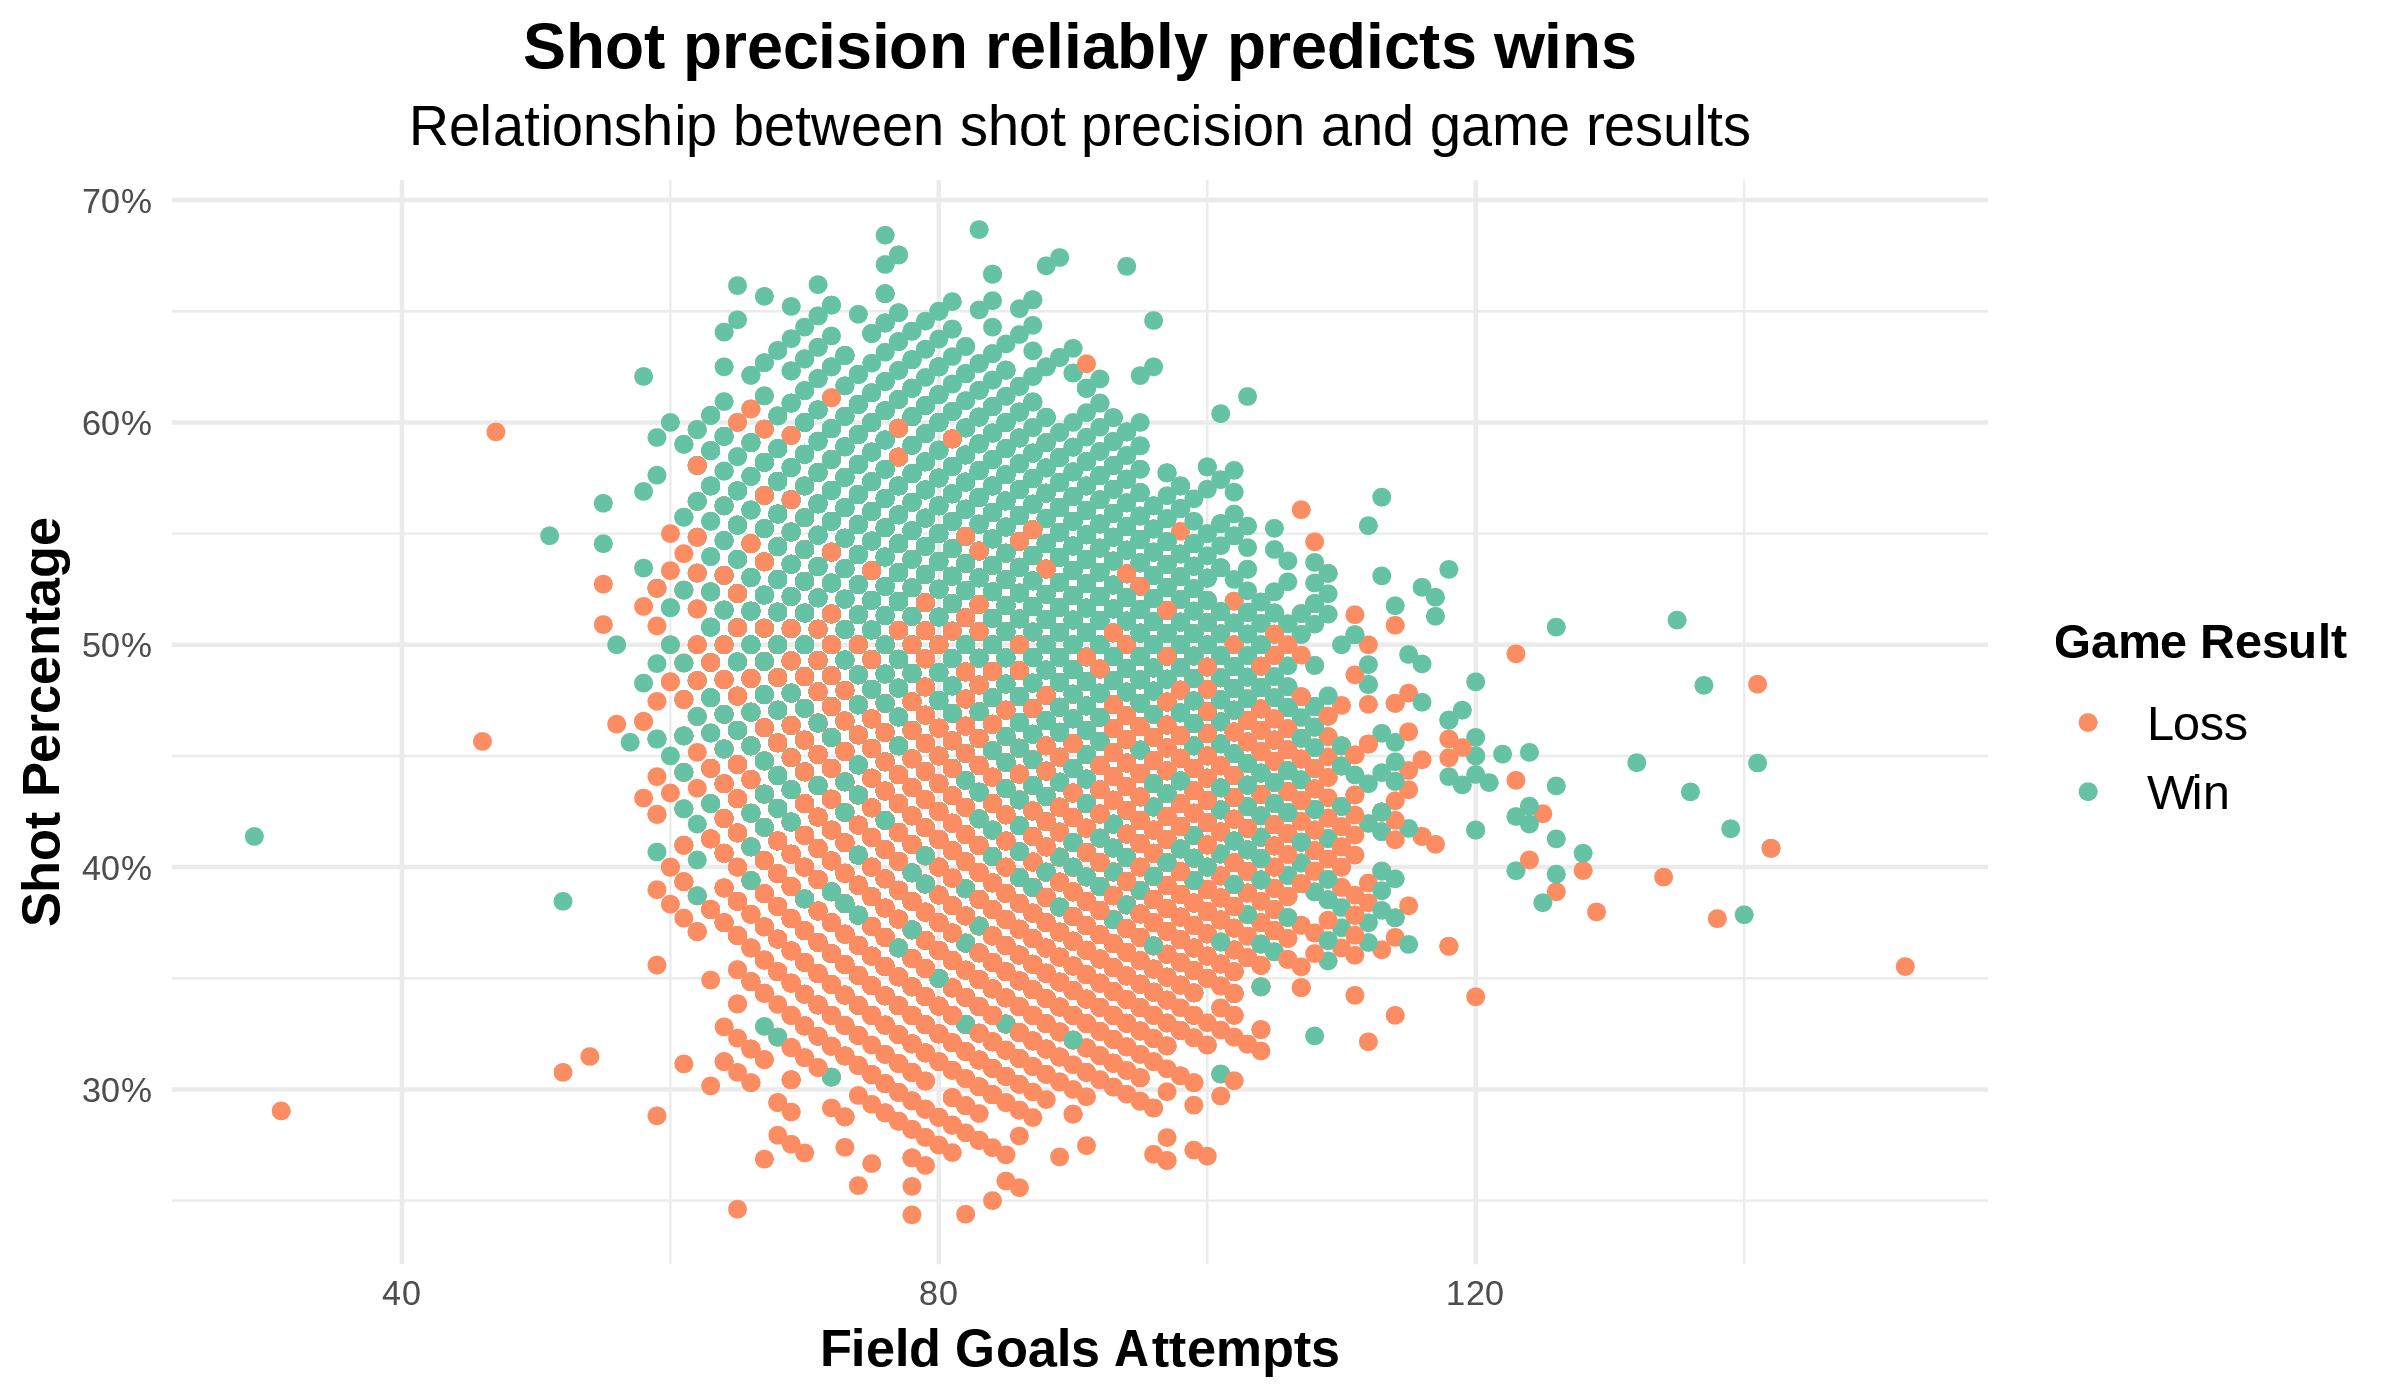
\includegraphics[width=0.49\linewidth]{latex/plotspres/plot_5} }\subfloat[3PT precision relationship with game results\label{fig:fgpred-2}]{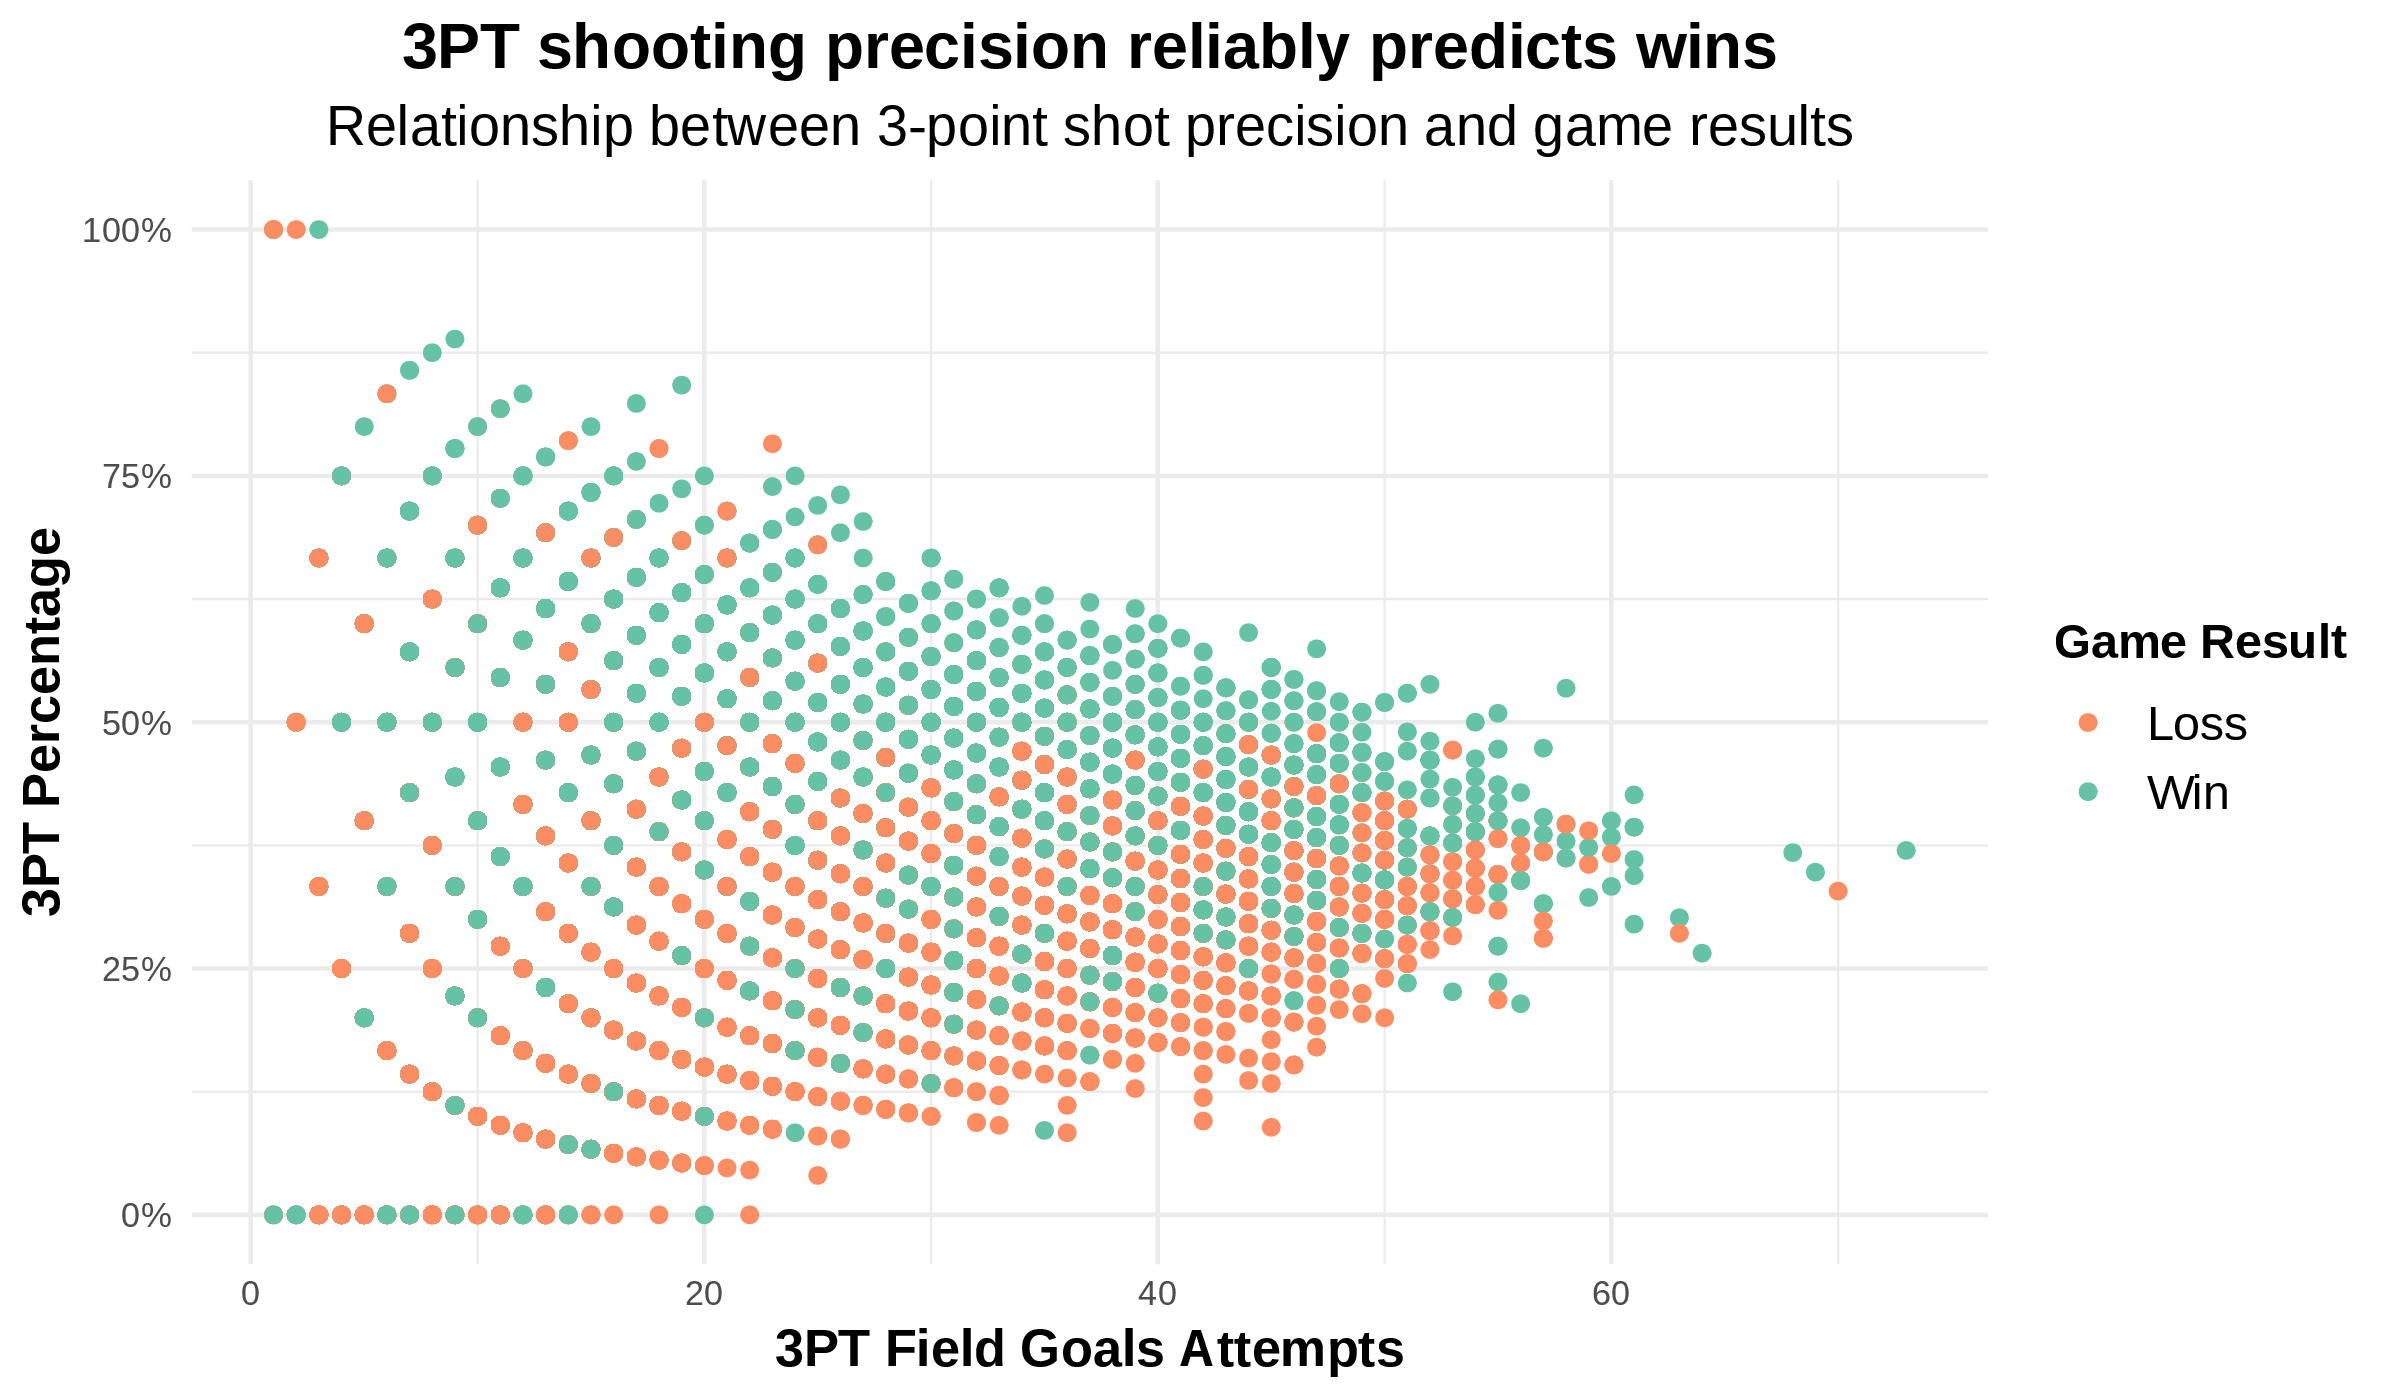
\includegraphics[width=0.49\linewidth]{latex/plotspres/plot_6} }

}

\caption{Role of shot precision in games predictions}\label{fig:fgpred}
\end{figure}
\end{frame}

\hypertarget{methodology}{%
\section{Methodology}\label{methodology}}

\begin{frame}[fragile]{Methodology}
Our methodology centers around the idea of integrating various types of
statistical modeling to predict NBA game outcomes. A key component of
our approach is the use of the ``Expected Value'' (\texttt{EV}) feature,
which we derive from the NBA shots dataset and which represents a given
shot type's expected efficiency based on data from the past 20 years. In
our analysis, we are mostly interested in seeing whether \texttt{EV} is
useful as a companion to field goal accuracy metrics, and then whether
it can also be useful as a predictor for game results on its own.
\end{frame}

\begin{frame}[fragile]{Variables selection}
\protect\hypertarget{variables-selection}{}
Our outcome variable is binary, reflecting whether or not the home team
won the game. Therefore, for each predictor statistic, we incorporate
both the home and away team's data. Besides the \texttt{EV} feature, the
predictors also include field goal precision (\texttt{FG\_PCT}), 3-point
FG precision (\texttt{FG3\_PCT}), free throw precision
(\texttt{FT\_PCT}), assists (\texttt{AST}), and rebounds (\texttt{REB}),
for both the home and away teams.

However, in assessing the prediction improvement yielded by the
\texttt{EV} feature, we may choose to exclude field goal statistics
(\texttt{FG}, \texttt{FG3}). Including these variables might skew the
analysis and overshadow the contribution of other variables, such as the
\texttt{EV} feature, therefore we fit models that both include and omit
field goal statistics.
\end{frame}

\begin{frame}{Predictive modeling techniques}
\protect\hypertarget{predictive-modeling-techniques}{}
We use two types of statistical models in our analysis: Logistic
Regression and Decision Trees.

\begin{itemize}
\item
  \emph{Logistic Regression}: The model predicts the probability of the
  positive class (in this case, the home team winning) as a logistic
  function of a linear combination of the predictors.
\item
  \emph{Decision Trees}: The model partitions the predictor space into
  several regions, and assigns a prediction to each region.
\end{itemize}

For both models, we partition our data into a training set (seasons up
to 2019) and a testing set (seasons after 2019). After fitting the
models to the training data, we assess their performance on the testing
data by employing \(k\)-fold cross-validation.
\end{frame}

\hypertarget{prediction-and-modeling}{%
\section{Prediction and modeling}\label{prediction-and-modeling}}

\begin{frame}[fragile]{Model fitting}
\protect\hypertarget{model-fitting}{}
In this section, we perform predictive modeling using logistic
regression and decision trees, and discuss the results by evaluating
performance metrics for each of the model fits.

When fitting a logistic regression model including all variables through
\(k\)-fold cross-validation, the result is that the efficiency of shots
for the home and away teams are statistically significant predictors at
any significance level. The coefficients for \texttt{EV\_home} and
\texttt{EV\_away} are positive and negative, respectively, indicating
that increased shot value for the home team and decreased shot value for
the away team both lead to a higher probability of a home team win. This
same pattern also holds for the other variables.
\end{frame}

\begin{frame}
\begin{figure}

{\centering 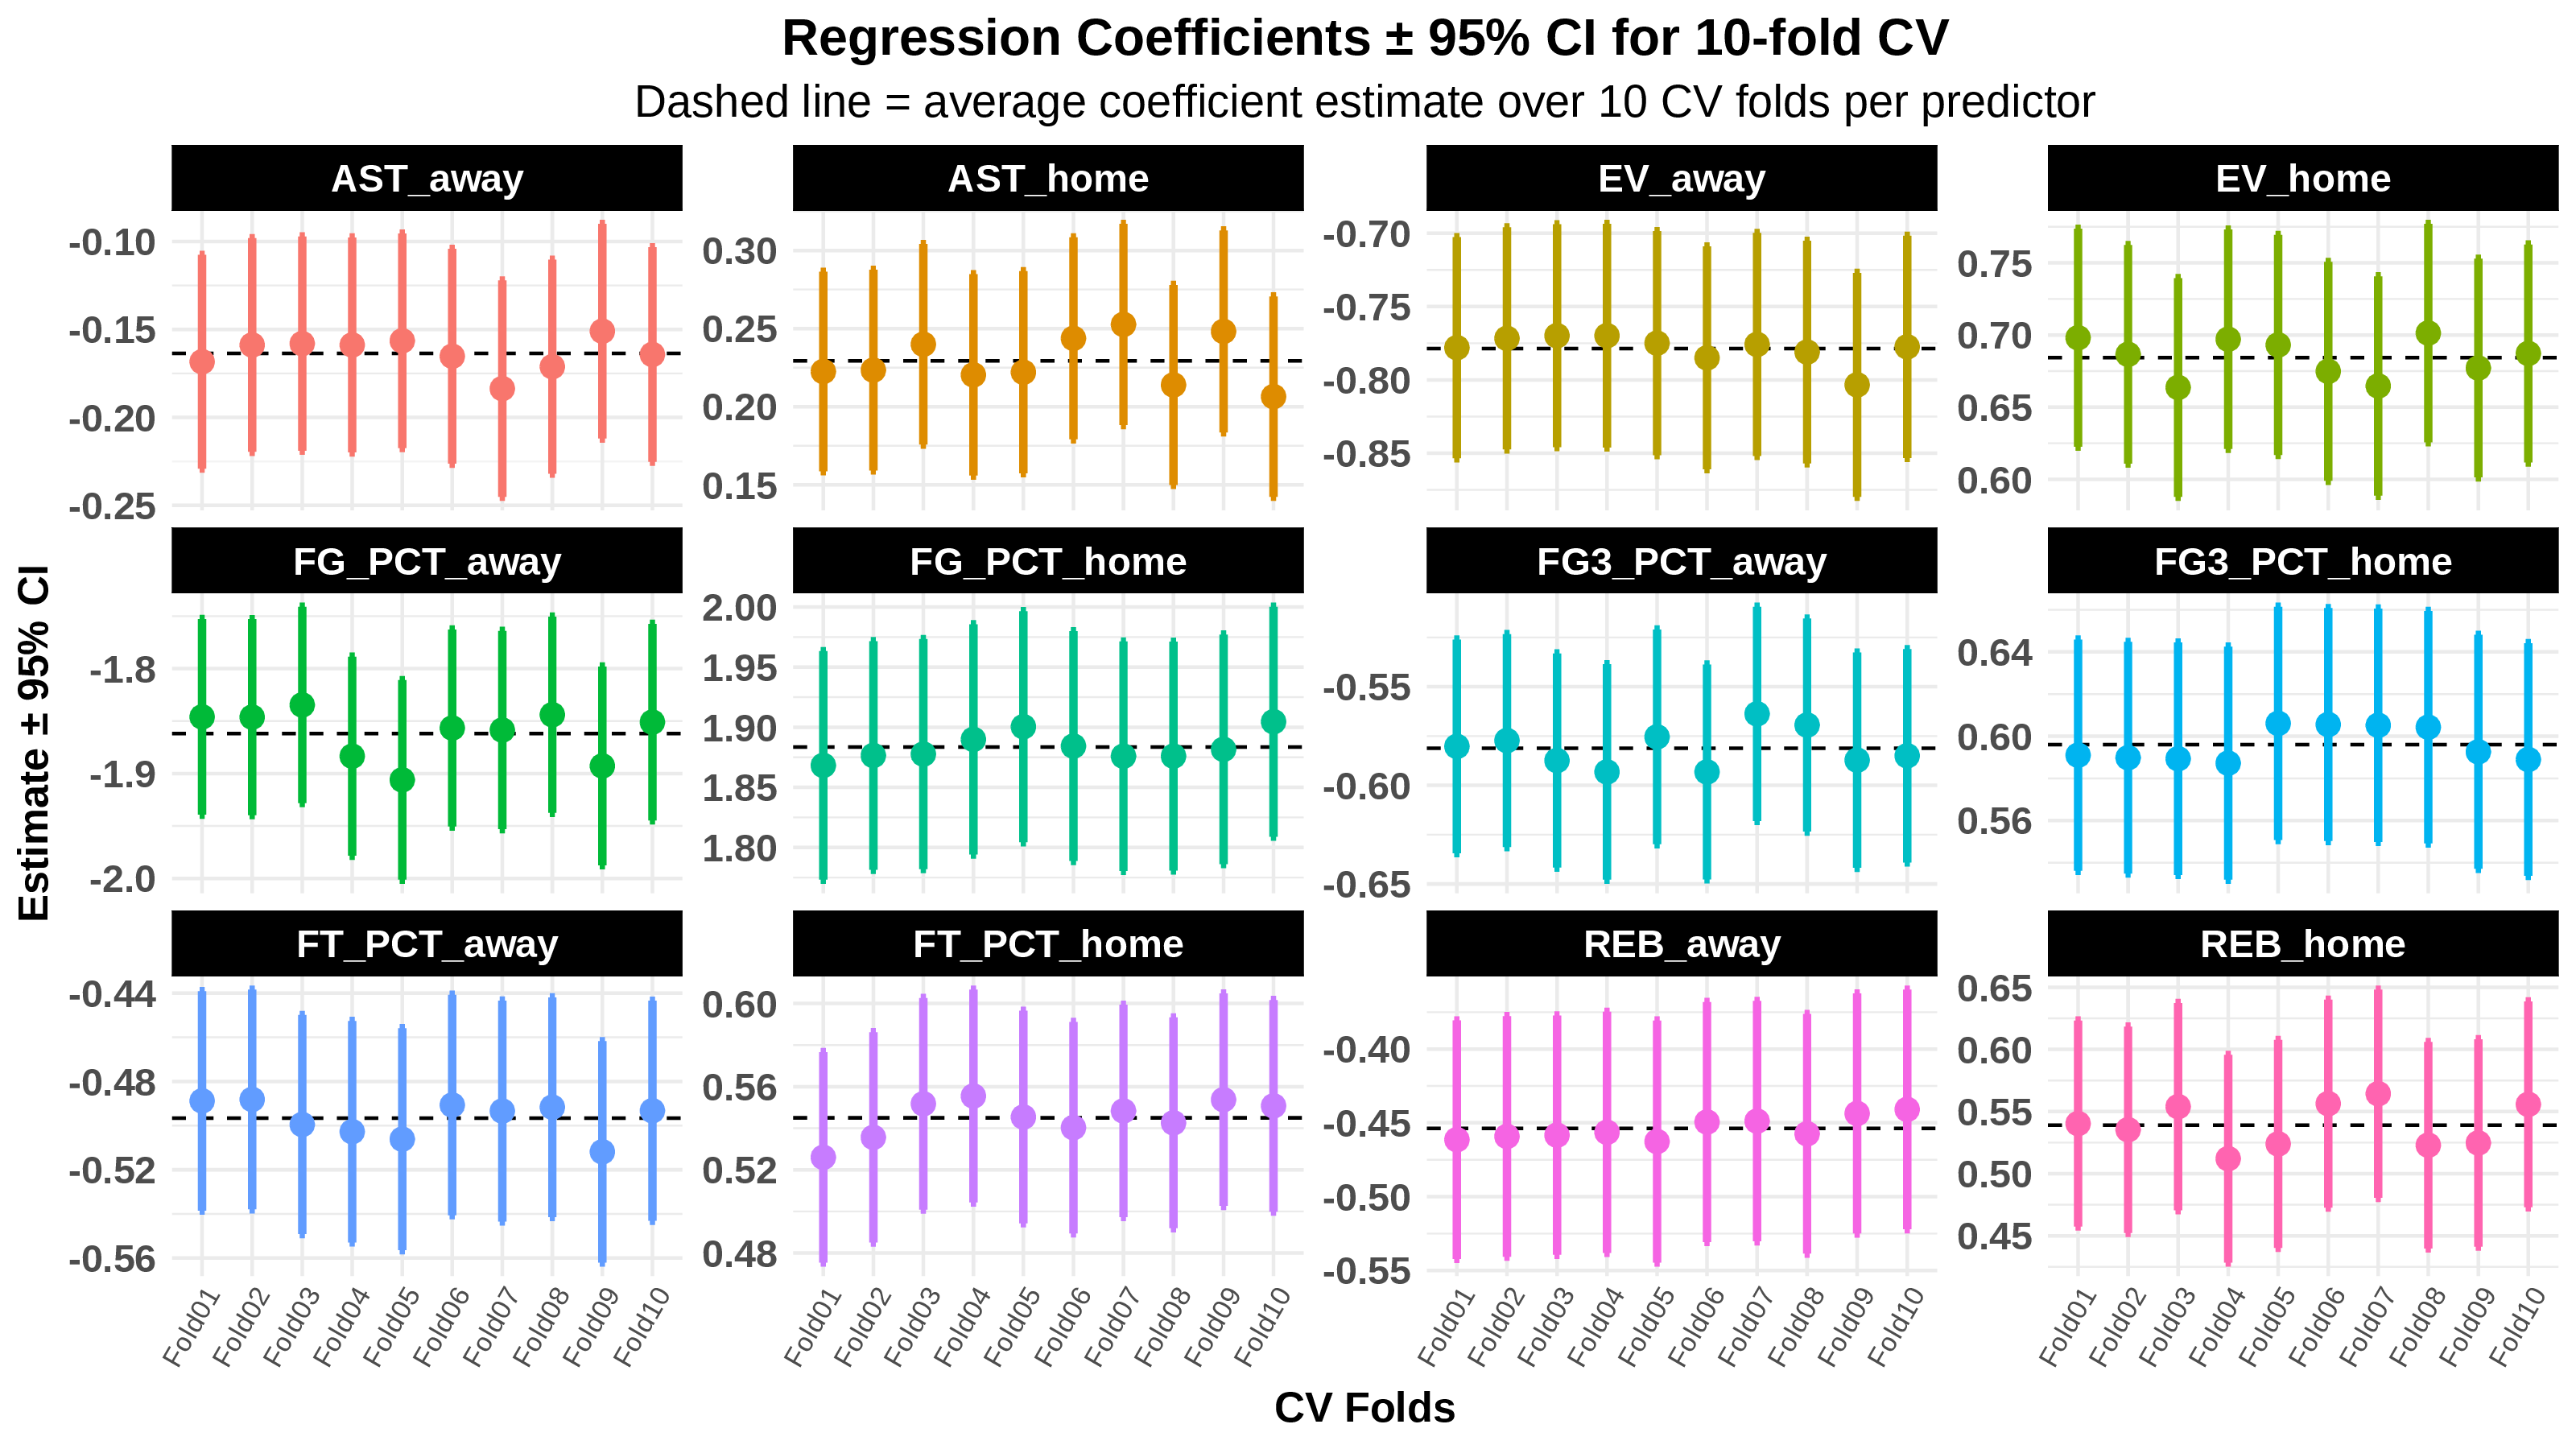
\includegraphics[width=1\linewidth]{latex/plotspres/plot_11} 

}

\caption{Coefficients for 10-fold full model cross-validation}\label{fig:regcoeffs}
\end{figure}
\end{frame}

\begin{frame}[fragile]
The decision tree model is subsequently fit to the training data, using
the same predictors. The variable importance plots rank the predictors
according to their weight in the decision tree models. Importance scores
are a way of scoring how useful each feature is for creating splits in
our data.

When we remove the field goal statistics from the model, the decision
tree uses \texttt{AST}, \texttt{EV}, and \texttt{REB} as primary splits.
The importance of these variables is confirmed in the variable
importance plot without FGs, shown as follows. From here, we can see
that the role of the \texttt{EV\_home} and \texttt{EV\_away} statistics
is quite important in the decisions adopted by the tree model.
\end{frame}

\begin{frame}
\begin{figure}

{\centering 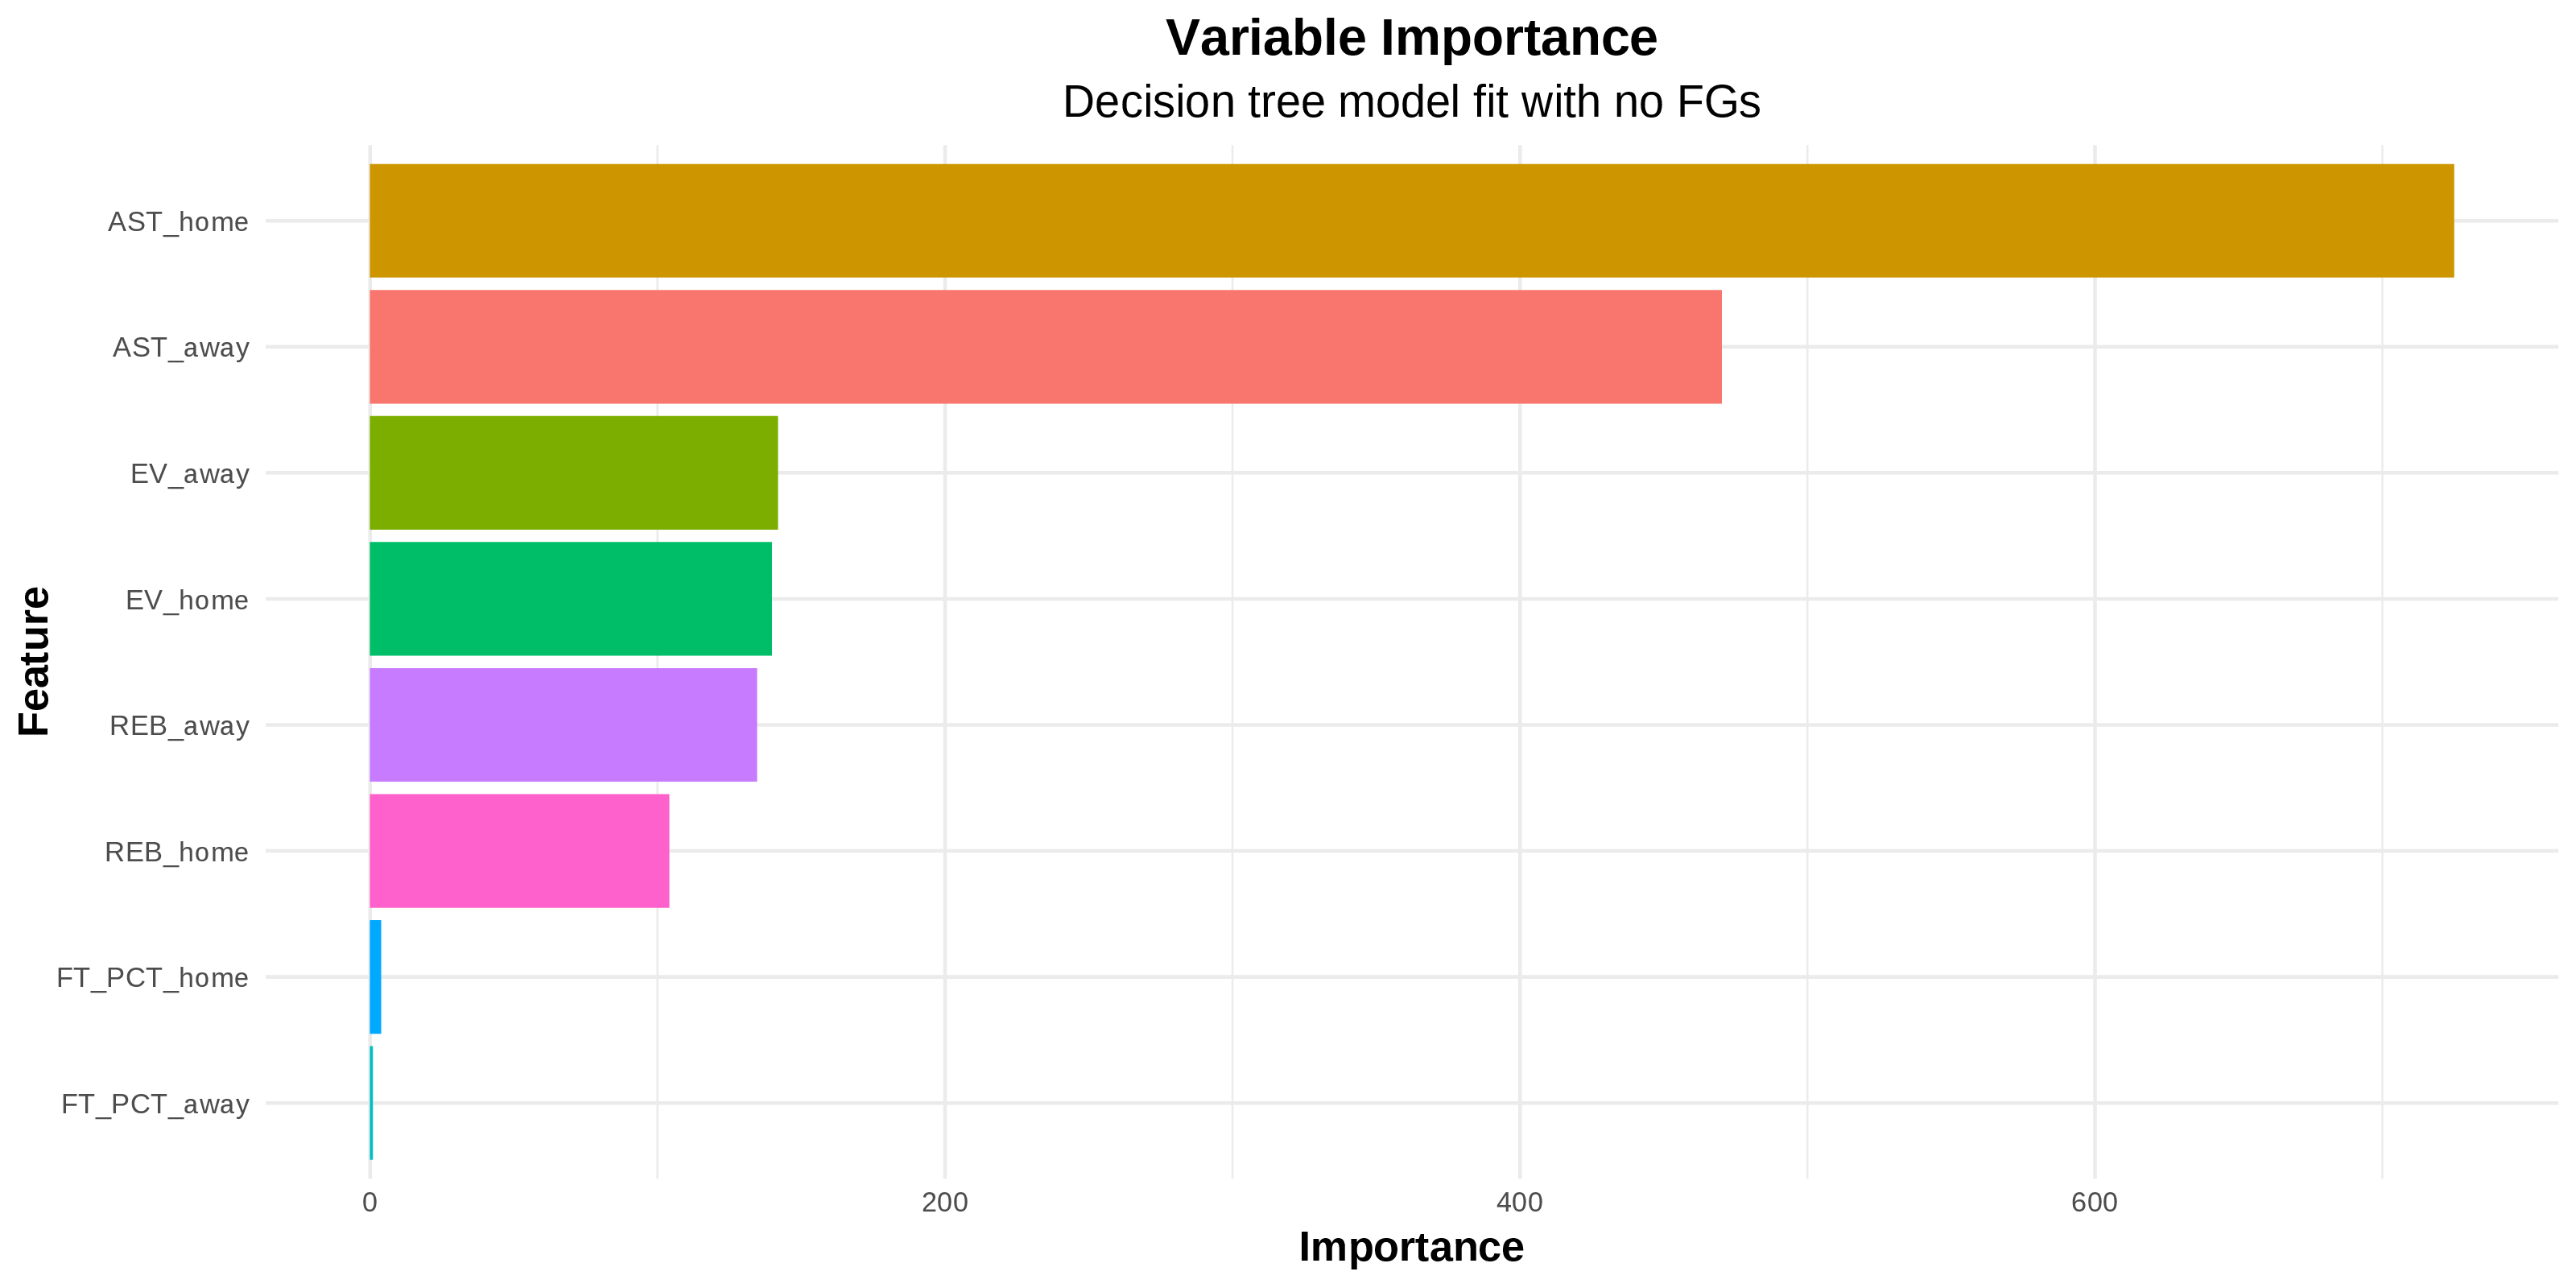
\includegraphics[width=1\linewidth]{latex/plotspres/plot_10} 

}

\caption{Variable Importance plot for model without shooting variables}\label{fig:vipnofg}
\end{figure}
\end{frame}

\begin{frame}{Model evaluation metrics}
\protect\hypertarget{model-evaluation-metrics}{}
In order to evaluate our models, we can show a number of metrics that
all evaluate the quality of classification.

\begin{itemize}
\item
  \emph{Cohen's Kappa (\(\kappa\))}: It gauges the level of agreement
  between the predicted and actual classes beyond what would be expected
  by chance.
\item
  \emph{F-measure (\(F\))}: It is the harmonic mean of precision and
  recall, which provides a balanced measure especially useful in uneven
  class distribution scenarios.
\item
  \emph{ROC AUC}: It represents a model's ability to distinguish between
  classes, with an AUC value between 0 (100\% wrong predictions) and 1
  (100\% correct predictions).
\end{itemize}
\end{frame}

\begin{frame}
The model metrics comparison shows that logistic regression models
outperform decision tree models in terms of all metrics, regardless of
whether field goal statistics are included or not.

\begin{figure}

{\centering 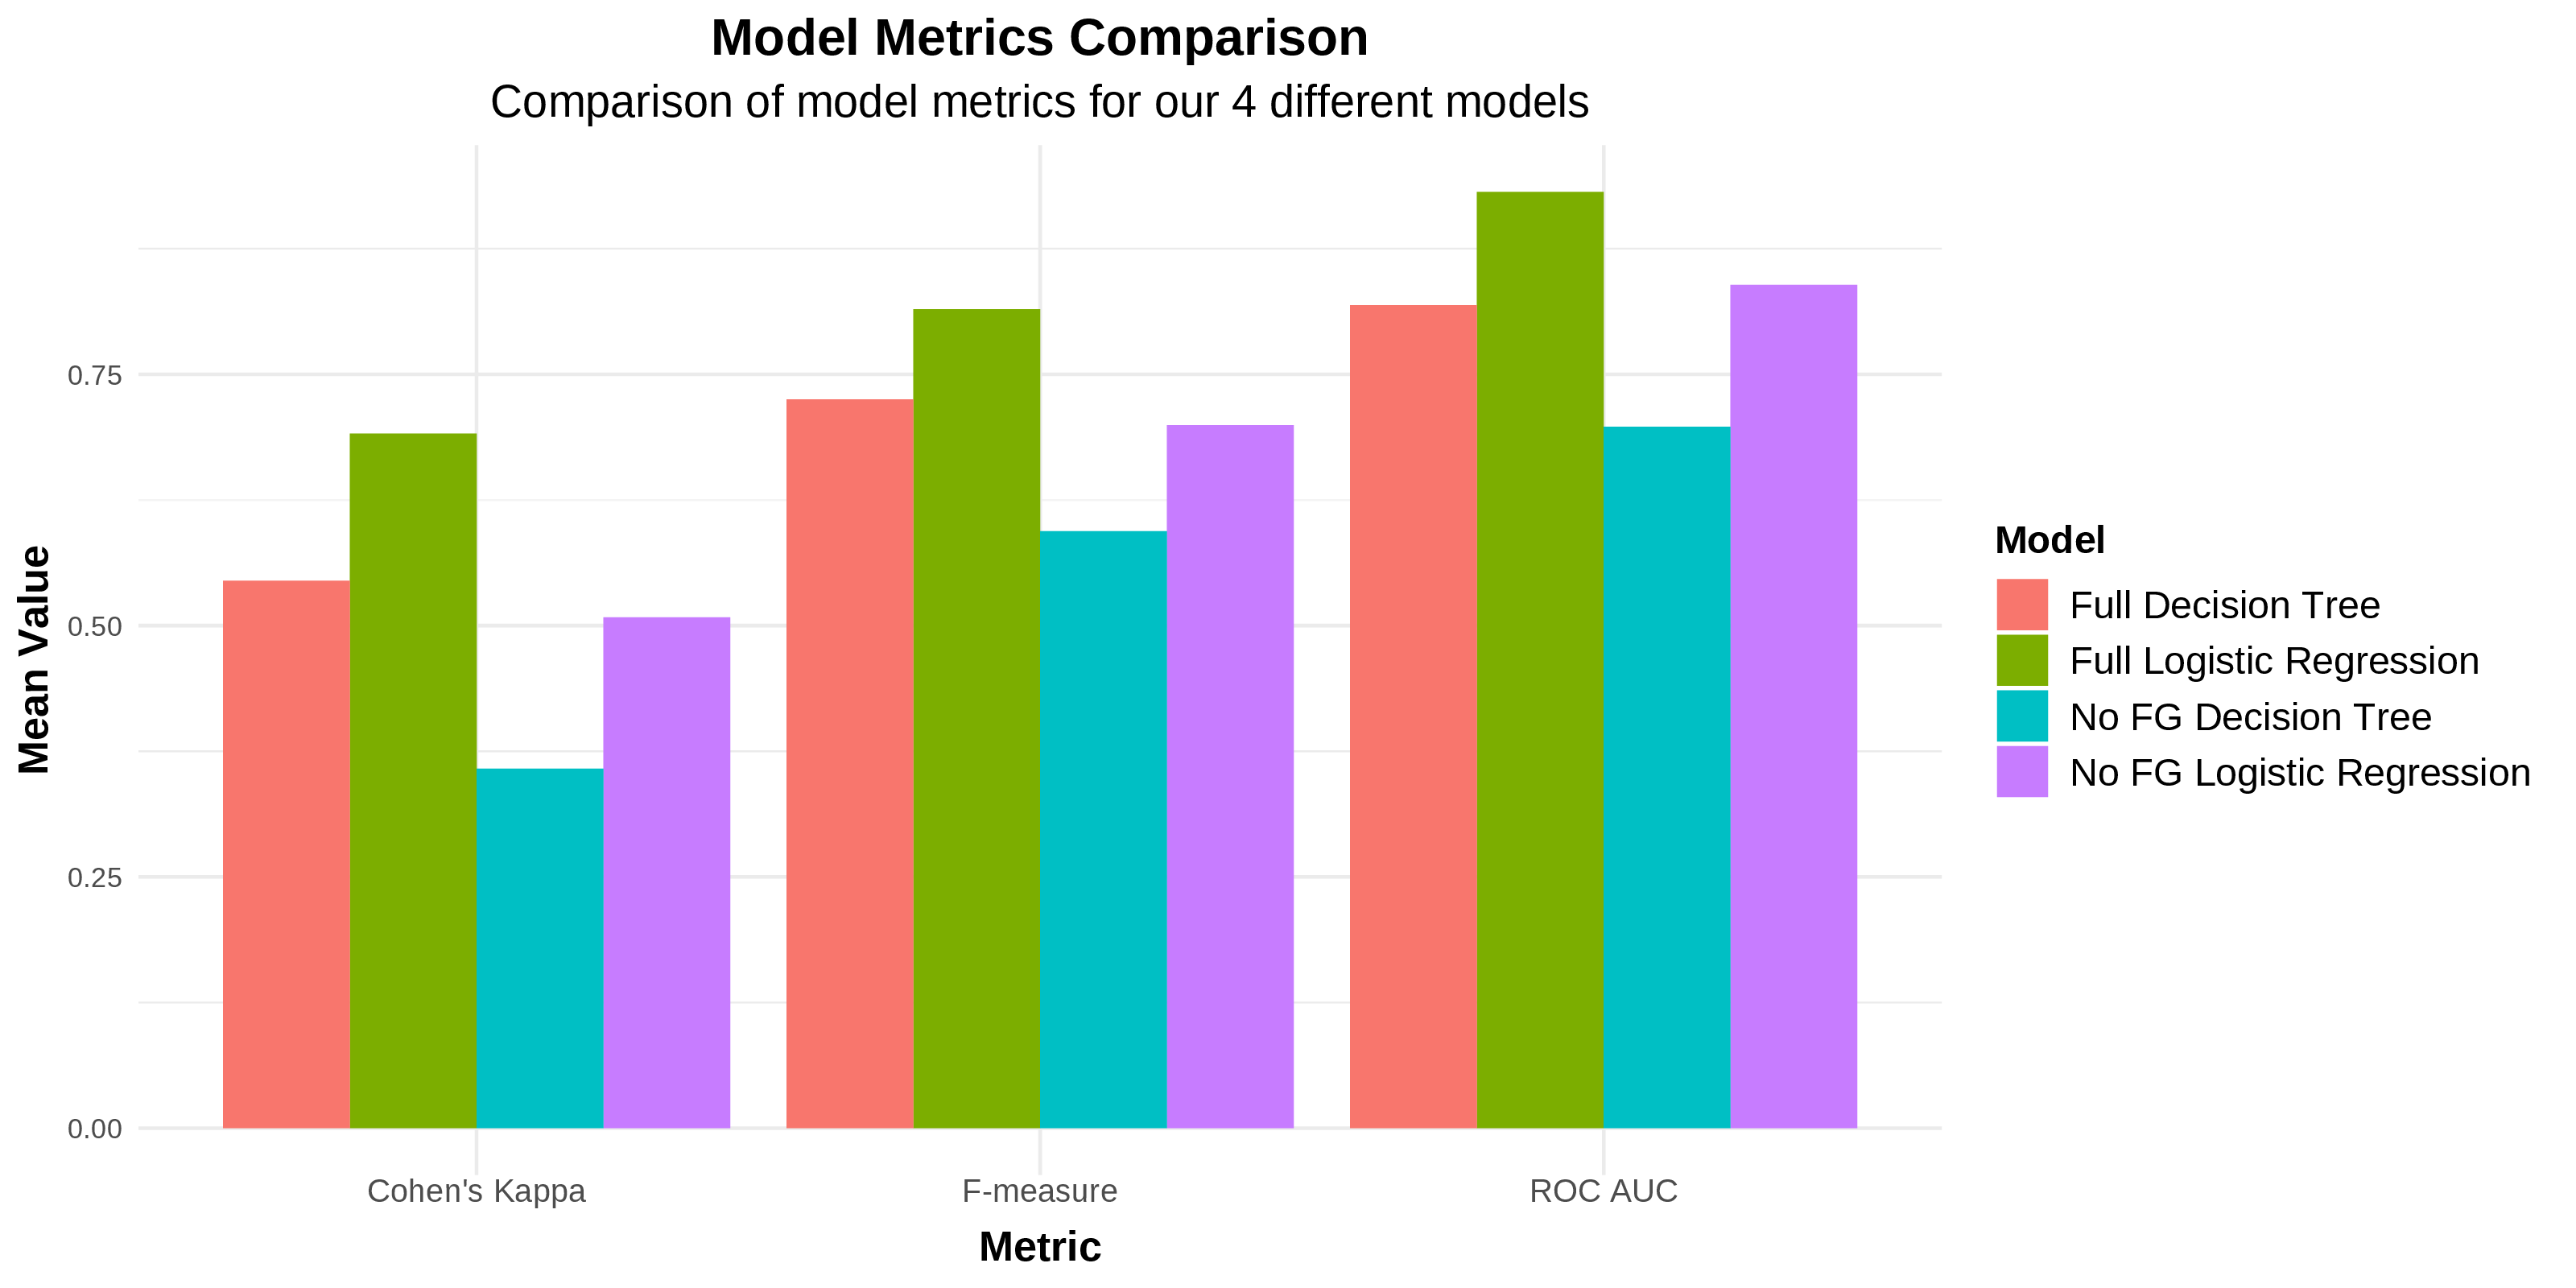
\includegraphics[width=1\linewidth]{latex/plotspres/plot_12} 

}

\caption{Comparison of model metrics for 4 different models}\label{fig:metricsplot}
\end{figure}
\end{frame}

\hypertarget{conclusions}{%
\section{Conclusions}\label{conclusions}}

\begin{frame}{Conclusions}
In summary, our analysis demonstrates that including the efficiency of
shots that a team takes as an explanatory variable can enhance the
prediction of NBA game outcomes.

However, a crucial limitation is that our predictions are retrospective
in nature. The models developed in this study are based on post-game
data, meaning they aim to explain the key components that influenced a
game's outcome, rather than forecasting future results.

Overall, while this research offers some insights into predicting NBA
game outcomes, there is significant scope for refinement. Future
research could benefit from utilizing a different modeling approach.
\end{frame}

\end{document}
